\chapter{Implementation}
\label{chapter:implementation}

% Miten ratkaisin ongelman?
% Arkkitehtuuri
% Työvoita
% Teknologia
% Eteen tulleet ongelmat toteutuksessa
% EI ohjelmadokumentti!

Here we describe how the methods are implemented to achieve the 
clustering. First we describe how the raw text data is 
pre-processed 

We implemented the workflow for clustering using Python's 
\texttt{scikit-learn} package completed with 
pre-processing managed with \texttt{doit} workflow. See Figure 
\ref{fig:wf} for the workflow graph.

\begin{figure}[ht]
  \begin{center}    
    % Graphic for TeX using PGF
% Title: /home/jlehtonen/nextcloud/synkronoitu/dippa/clustering/doc/images/workflow.dia
% Creator: Dia v0.97.3
% CreationDate: Mon Dec  9 05:57:48 2019
% For: jlehtonen
% \usepackage{tikz}
% The following commands are not supported in PSTricks at present
% We define them conditionally, so when they are implemented,
% this pgf file will use them.
\ifx\du\undefined
  \newlength{\du}
\fi
\setlength{\du}{15\unitlength}
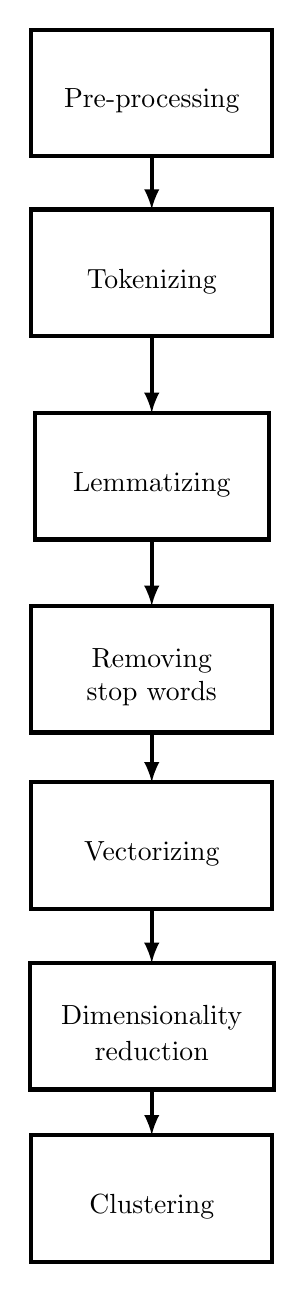
\begin{tikzpicture}
\pgftransformxscale{1.000000}
\pgftransformyscale{-1.000000}
\definecolor{dialinecolor}{rgb}{0.000000, 0.000000, 0.000000}
\pgfsetstrokecolor{dialinecolor}
\definecolor{dialinecolor}{rgb}{1.000000, 1.000000, 1.000000}
\pgfsetfillcolor{dialinecolor}
\definecolor{dialinecolor}{rgb}{1.000000, 1.000000, 1.000000}
\pgfsetfillcolor{dialinecolor}
\fill (5.932500\du,3.900000\du)--(5.932500\du,6.950000\du)--(11.730000\du,6.950000\du)--(11.730000\du,3.900000\du)--cycle;
\pgfsetlinewidth{0.100000\du}
\pgfsetdash{}{0pt}
\pgfsetdash{}{0pt}
\pgfsetmiterjoin
\definecolor{dialinecolor}{rgb}{0.000000, 0.000000, 0.000000}
\pgfsetstrokecolor{dialinecolor}
\draw (5.932500\du,3.900000\du)--(5.932500\du,6.950000\du)--(11.730000\du,6.950000\du)--(11.730000\du,3.900000\du)--cycle;
% setfont left to latex
\definecolor{dialinecolor}{rgb}{0.000000, 0.000000, 0.000000}
\pgfsetstrokecolor{dialinecolor}
\node at (8.831250\du,5.620000\du){Pre-processing};
% setfont left to latex
\definecolor{dialinecolor}{rgb}{0.000000, 0.000000, 0.000000}
\pgfsetstrokecolor{dialinecolor}
\node[anchor=west] at (8.831250\du,5.425000\du){};
\definecolor{dialinecolor}{rgb}{1.000000, 1.000000, 1.000000}
\pgfsetfillcolor{dialinecolor}
\fill (5.932500\du,8.230000\du)--(5.932500\du,11.280000\du)--(11.730000\du,11.280000\du)--(11.730000\du,8.230000\du)--cycle;
\pgfsetlinewidth{0.100000\du}
\pgfsetdash{}{0pt}
\pgfsetdash{}{0pt}
\pgfsetmiterjoin
\definecolor{dialinecolor}{rgb}{0.000000, 0.000000, 0.000000}
\pgfsetstrokecolor{dialinecolor}
\draw (5.932500\du,8.230000\du)--(5.932500\du,11.280000\du)--(11.730000\du,11.280000\du)--(11.730000\du,8.230000\du)--cycle;
% setfont left to latex
\definecolor{dialinecolor}{rgb}{0.000000, 0.000000, 0.000000}
\pgfsetstrokecolor{dialinecolor}
\node at (8.831250\du,9.950000\du){};
% setfont left to latex
\definecolor{dialinecolor}{rgb}{0.000000, 0.000000, 0.000000}
\pgfsetstrokecolor{dialinecolor}
\node at (8.831250\du,9.976250\du){Tokenizing};
% setfont left to latex
\definecolor{dialinecolor}{rgb}{0.000000, 0.000000, 0.000000}
\pgfsetstrokecolor{dialinecolor}
\node[anchor=west] at (8.840594\du,17.305000\du){};
\definecolor{dialinecolor}{rgb}{1.000000, 1.000000, 1.000000}
\pgfsetfillcolor{dialinecolor}
\fill (6.014375\du,13.130000\du)--(6.014375\du,16.180000\du)--(11.648125\du,16.180000\du)--(11.648125\du,13.130000\du)--cycle;
\pgfsetlinewidth{0.100000\du}
\pgfsetdash{}{0pt}
\pgfsetdash{}{0pt}
\pgfsetmiterjoin
\definecolor{dialinecolor}{rgb}{0.000000, 0.000000, 0.000000}
\pgfsetstrokecolor{dialinecolor}
\draw (6.014375\du,13.130000\du)--(6.014375\du,16.180000\du)--(11.648125\du,16.180000\du)--(11.648125\du,13.130000\du)--cycle;
% setfont left to latex
\definecolor{dialinecolor}{rgb}{0.000000, 0.000000, 0.000000}
\pgfsetstrokecolor{dialinecolor}
\node at (8.831250\du,14.850000\du){Lemmatizing};
\definecolor{dialinecolor}{rgb}{1.000000, 1.000000, 1.000000}
\pgfsetfillcolor{dialinecolor}
\fill (5.932500\du,17.780000\du)--(5.932500\du,20.830000\du)--(11.730000\du,20.830000\du)--(11.730000\du,17.780000\du)--cycle;
\pgfsetlinewidth{0.100000\du}
\pgfsetdash{}{0pt}
\pgfsetdash{}{0pt}
\pgfsetmiterjoin
\definecolor{dialinecolor}{rgb}{0.000000, 0.000000, 0.000000}
\pgfsetstrokecolor{dialinecolor}
\draw (5.932500\du,17.780000\du)--(5.932500\du,20.830000\du)--(11.730000\du,20.830000\du)--(11.730000\du,17.780000\du)--cycle;
% setfont left to latex
\definecolor{dialinecolor}{rgb}{0.000000, 0.000000, 0.000000}
\pgfsetstrokecolor{dialinecolor}
\node at (8.831250\du,19.100000\du){Removing};
% setfont left to latex
\definecolor{dialinecolor}{rgb}{0.000000, 0.000000, 0.000000}
\pgfsetstrokecolor{dialinecolor}
\node at (8.831250\du,19.900000\du){stop words};
\definecolor{dialinecolor}{rgb}{1.000000, 1.000000, 1.000000}
\pgfsetfillcolor{dialinecolor}
\fill (5.932500\du,22.030000\du)--(5.932500\du,25.080000\du)--(11.730000\du,25.080000\du)--(11.730000\du,22.030000\du)--cycle;
\pgfsetlinewidth{0.100000\du}
\pgfsetdash{}{0pt}
\pgfsetdash{}{0pt}
\pgfsetmiterjoin
\definecolor{dialinecolor}{rgb}{0.000000, 0.000000, 0.000000}
\pgfsetstrokecolor{dialinecolor}
\draw (5.932500\du,22.030000\du)--(5.932500\du,25.080000\du)--(11.730000\du,25.080000\du)--(11.730000\du,22.030000\du)--cycle;
% setfont left to latex
\definecolor{dialinecolor}{rgb}{0.000000, 0.000000, 0.000000}
\pgfsetstrokecolor{dialinecolor}
\node at (8.831250\du,23.750000\du){Vectorizing};
\definecolor{dialinecolor}{rgb}{1.000000, 1.000000, 1.000000}
\pgfsetfillcolor{dialinecolor}
\fill (5.892500\du,26.380000\du)--(5.892500\du,29.430000\du)--(11.770000\du,29.430000\du)--(11.770000\du,26.380000\du)--cycle;
\pgfsetlinewidth{0.100000\du}
\pgfsetdash{}{0pt}
\pgfsetdash{}{0pt}
\pgfsetmiterjoin
\definecolor{dialinecolor}{rgb}{0.000000, 0.000000, 0.000000}
\pgfsetstrokecolor{dialinecolor}
\draw (5.892500\du,26.380000\du)--(5.892500\du,29.430000\du)--(11.770000\du,29.430000\du)--(11.770000\du,26.380000\du)--cycle;
% setfont left to latex
\definecolor{dialinecolor}{rgb}{0.000000, 0.000000, 0.000000}
\pgfsetstrokecolor{dialinecolor}
\node at (8.831250\du,27.700000\du){Dimensionality};
% setfont left to latex
\definecolor{dialinecolor}{rgb}{0.000000, 0.000000, 0.000000}
\pgfsetstrokecolor{dialinecolor}
\node at (8.831250\du,28.500000\du){reduction};
\pgfsetlinewidth{0.100000\du}
\pgfsetdash{}{0pt}
\pgfsetdash{}{0pt}
\pgfsetbuttcap
{
\definecolor{dialinecolor}{rgb}{0.000000, 0.000000, 0.000000}
\pgfsetfillcolor{dialinecolor}
% was here!!!
\pgfsetarrowsend{latex}
\definecolor{dialinecolor}{rgb}{0.000000, 0.000000, 0.000000}
\pgfsetstrokecolor{dialinecolor}
\draw (8.831250\du,6.950000\du)--(8.831250\du,8.230000\du);
}
\pgfsetlinewidth{0.100000\du}
\pgfsetdash{}{0pt}
\pgfsetdash{}{0pt}
\pgfsetbuttcap
{
\definecolor{dialinecolor}{rgb}{0.000000, 0.000000, 0.000000}
\pgfsetfillcolor{dialinecolor}
% was here!!!
\pgfsetarrowsend{latex}
\definecolor{dialinecolor}{rgb}{0.000000, 0.000000, 0.000000}
\pgfsetstrokecolor{dialinecolor}
\draw (8.831250\du,11.280000\du)--(8.831250\du,13.130000\du);
}
\pgfsetlinewidth{0.100000\du}
\pgfsetdash{}{0pt}
\pgfsetdash{}{0pt}
\pgfsetbuttcap
{
\definecolor{dialinecolor}{rgb}{0.000000, 0.000000, 0.000000}
\pgfsetfillcolor{dialinecolor}
% was here!!!
\pgfsetarrowsend{latex}
\definecolor{dialinecolor}{rgb}{0.000000, 0.000000, 0.000000}
\pgfsetstrokecolor{dialinecolor}
\draw (8.831250\du,16.180000\du)--(8.831250\du,17.780000\du);
}
\pgfsetlinewidth{0.100000\du}
\pgfsetdash{}{0pt}
\pgfsetdash{}{0pt}
\pgfsetbuttcap
{
\definecolor{dialinecolor}{rgb}{0.000000, 0.000000, 0.000000}
\pgfsetfillcolor{dialinecolor}
% was here!!!
\pgfsetarrowsend{latex}
\definecolor{dialinecolor}{rgb}{0.000000, 0.000000, 0.000000}
\pgfsetstrokecolor{dialinecolor}
\draw (8.831250\du,20.830000\du)--(8.831250\du,22.030000\du);
}
% setfont left to latex
\definecolor{dialinecolor}{rgb}{0.000000, 0.000000, 0.000000}
\pgfsetstrokecolor{dialinecolor}
\node[anchor=west] at (8.831250\du,27.905000\du){};
% setfont left to latex
\definecolor{dialinecolor}{rgb}{0.000000, 0.000000, 0.000000}
\pgfsetstrokecolor{dialinecolor}
\node[anchor=west] at (8.831250\du,27.905000\du){};
\definecolor{dialinecolor}{rgb}{1.000000, 1.000000, 1.000000}
\pgfsetfillcolor{dialinecolor}
\fill (5.932500\du,30.530000\du)--(5.932500\du,33.580000\du)--(11.730000\du,33.580000\du)--(11.730000\du,30.530000\du)--cycle;
\pgfsetlinewidth{0.100000\du}
\pgfsetdash{}{0pt}
\pgfsetdash{}{0pt}
\pgfsetmiterjoin
\definecolor{dialinecolor}{rgb}{0.000000, 0.000000, 0.000000}
\pgfsetstrokecolor{dialinecolor}
\draw (5.932500\du,30.530000\du)--(5.932500\du,33.580000\du)--(11.730000\du,33.580000\du)--(11.730000\du,30.530000\du)--cycle;
% setfont left to latex
\definecolor{dialinecolor}{rgb}{0.000000, 0.000000, 0.000000}
\pgfsetstrokecolor{dialinecolor}
\node at (8.831250\du,32.250000\du){Clustering};
% setfont left to latex
\definecolor{dialinecolor}{rgb}{0.000000, 0.000000, 0.000000}
\pgfsetstrokecolor{dialinecolor}
\node[anchor=west] at (8.831250\du,32.055000\du){};
\pgfsetlinewidth{0.100000\du}
\pgfsetdash{}{0pt}
\pgfsetdash{}{0pt}
\pgfsetbuttcap
{
\definecolor{dialinecolor}{rgb}{0.000000, 0.000000, 0.000000}
\pgfsetfillcolor{dialinecolor}
% was here!!!
\pgfsetarrowsend{latex}
\definecolor{dialinecolor}{rgb}{0.000000, 0.000000, 0.000000}
\pgfsetstrokecolor{dialinecolor}
\draw (8.831250\du,25.080000\du)--(8.831250\du,26.380000\du);
}
\pgfsetlinewidth{0.100000\du}
\pgfsetdash{}{0pt}
\pgfsetdash{}{0pt}
\pgfsetbuttcap
{
\definecolor{dialinecolor}{rgb}{0.000000, 0.000000, 0.000000}
\pgfsetfillcolor{dialinecolor}
% was here!!!
\pgfsetarrowsend{latex}
\definecolor{dialinecolor}{rgb}{0.000000, 0.000000, 0.000000}
\pgfsetstrokecolor{dialinecolor}
\draw (8.831250\du,29.430000\du)--(8.831250\du,30.530000\du);
}
\end{tikzpicture}

    \caption{The workflow of the clustering.}
    \label{fig:wf}
  \end{center}
\end{figure}

\section{Preprocessing}
First data was read from raw files obtained from publishers. 
%(Actually YL probably also preprocessed data before passing it 
% to me.)
We choose to omit some metadata fields from the analysis (cf. 
section \ref{section:metadata}). Fields \emph{journal}, 
\emph{issn} and \emph{the field of science} were omitted because 
they exhibit the existing classification whereas we wanted an 
alternative one. The field \emph{year} is irrelevant here as our 
analysis doesn't include temporal aspect. The field 
\emph{references} was also left out because the references 
would've needed different treatment and more theoretical research 
on how to be used as features for clustering 
% \fixme{Täydennä perustelua}.

We choose to keep \emph{title}, \emph{abstract} and 
\emph{keyword} fields. All the title, abstract and author 
provided keywords are original data of the publication without 
any external interpretation. We also choose to keep the automatic 
publisher inferred keywords (``\texttt{Avainsana 
(KeywordPlus)}'') because these can be seen as concentration of 
publication data by some text analysis algorithm. The algorithm is 
unknown here but we assume that the aim of the these keywords is 
also to describe the publication as well as possible. 
% \fixme{Paranna perustelua} 
Terms in keyword fields were concatenated into combined terms: 
``allergic\_contact\_dermatitis''. This is related to the counting 
of words in a metadata and will be explained soon. The kept 
metadata fields were read into a dictionary and data saved in 
intermediate files.

\section{Tokenizing}
The metadata in chosen fields was then tokenized with whitespace 
and punctuation other than perioids separating the tokens (words). 
We get for example ``\emph{Pluto is a smart dog}'' $\rightarrow$ 
``\emph{Pluto}'', ``\emph{is}'', ``\emph{a}'', ``\emph{smart}'' 
and ``\emph{dog}'' (the \emph{bag of words} representation).
Alternatively we could form n-grams out of the text to preserve 
the meaning of combined terms. For example when tokenizing 
``\emph{allergic contact dermatitis}'', instead of 
``\emph{allergic}'', ``\emph{contact}'' and 
``\emph{dermatitis}'' we would get ``\emph{allergic contact}'' 
and ``\emph{contact dermatitis}''. Here single words are called 
1-grams, word pairs are called 2-grams and so on. Counting the 
n-grams would expand the feature space n-fold though and we wanted 
to avoid the computational cost. 
% Koitetaan ottaa 2-grammit mukaan
% 29.4. 2-grammit 'future work' -osioon

\section{Lemmatizing}
After tokenizing the words we lemmatized them against WordNet 
lemmatizer \cite{noauthor_princeton_2010}.
% After parsing data is written to interim files.
We choose to remove all plain numbers from
data. Another option is to replace numbers with dummy '\#NUMBER'.
That could help separate natural sciences from humanities. Because 
we didn't have proper knowledge on the issue removal was chosen. 
We assumed that to be a more neutral way to treat them. 
% \fixme{How? Explain...}
If the lemmatizer didn't found the word in WordNet Lemmatizer 
database the word is returned unchanged. 
% \fixme{Huomioita lemmatisoinnin tuloksesta}

\section{Removing stop words}
Stop words were then removed after lemmatisation. We used Python's
\texttt{NLTK} module's English stop words 
combined with \texttt{scikit-learn's} stop words and our own stop 
word list consisting mainly standard publisher notices 
(\emph{``rights'', ``reserved''} and publising years). The stop 
word list included 352 words.


\section{Vectorizing}
After removing stop words the term frequencies were counted and 
normalized with inverse document frequencies (\emph{tf-idf} 
normalization). 
In this point we have the data vectorized.

We set the minimum document frequency, under which the terms 
having their \emph{tf-idf} value are ignored, to $min_df=2$, so 
two occurences. The maximum document frequency, over which the 
terms having their \emph{tf-idf} value are ignored, to 
$max_df=0.5$, so to 50 \% of the documents.
These cut-off values resulted in 7123 ignored terms and the 
feature space of 3372 terms. Terms that were filtered out as too 
frequent or too few were for example: ``haemoglobin\_a'', 
``jacobian\_matrix'', 
``parthenogenetic'', ``chelation\_by\_saccharide\_molecules'', 
``leg\_blood\_supply'', ``computational\_fluid\_dynamics'', 
``pigment'', ``hdtv'', ``nicotinic\_receptor''.

% \fixme{To verify these parameter values it would be interesting 
% to know the frequencies of the filtered-out terms. It didn't come 
% out straight from TfIdfVectroizer class used but taking different 
% levels of $min_df$ and $max_df$ could be used to view different 
% frequency groups.} Ei ehdi

%\fixme{Onko näissä esikäsittelyvaiheissa joitain parametreja 
%jonka suhteen tuloksia haluttaisiin tarkastella? Riittänee että 
%tokenointi ja lemmatisointi toimivat. Noissa sanatiheyden
%leikkausarvoissa min ja max-df voisi olla jotain.}


\section{Clustering}
When clustering with Ward's hierarchical clustering the 
interesting parameter values are the number of the clusters, 
the distance measure, the cluster connectivity measure, the 
number of the components ie. the amount of dimensionality 
reduction. 

To decide the number of clusters we experimented with the manually 
annotated data set described in section \ref{sec:ext_val}.
% Käsin luokitellun aineiston kuvaus
The validation set consists of Finnish publications from year 2000
from three different fields of science as categorized by WoS.
Two of the fields are closely related sub fields of computer
science: \emph{computer science: information systems} (CS-IS) and 
\emph{computer science: 
artificial intelligence} (CS-AI), while the third one, 
\emph{clinical neurology}, is more distant from those. There are 
$116$, $122$, $250$ publications labeled as belonging to fields 
CS-IS, CS-AI and clinical neurology respectively, and $31$ 
publications labeled as belonging to both CS-IS and CS-AI, 
totalling $519$ publications in our data.

% Huonojen näytteiden poisto
Publications were inspected by title, abstract, keywords, journal
and publisher assigned disciplines of the journal. Publications
with critically missing data, unclear discipline assignment and
heavily applied publications (eg. a publication describing the 
development of a virtual community and a community game platform)
were excluded from validation set. 
% Luokittelun varmistus käsin
We then checked with layman's reasoning if the WoS labeled 
discipline seemed plausible. Because of the journal based 
classification, most publications had more than one assigned 
discipline. Only the previously named three discipline labels were 
retained because we wanted to test if and how well our clustering 
method would cluster the samples compared to these three 
groups. We asked an another opinion of non-expert human 
reviewer for 37 the most ambiguous publications that could have 
been in more than one of our categories. 
For manually curated
validation set with discipline assignment and justifications for
possible exclusion see appendix \ref{chapter:first-appendix}.
% ``Väärin luokiteltujen uudelleen luokittelu''
In total $29$ publications were manually reclassified by either
choosing only one of two used classes or by assigning the 
publication to more fitting category by our judgement. After
excluding bad data and reclassifications we had a data set of 
$134$, $127$ and $194$ publications in CS-IS, CS-AI and clinical
neurology, respectively, totalling $455$ publications.

% Pitäisikö tämä olla jossain muualla?
% ``Väärin'' luokiteltujen uudelleen luokittelusta
The basic problem is that fields of science can not be 
defined so that they clearly differ from each other. Where one 
discipline end the other has already started like metallurgy and 
material science. Likewise, there are lots of publications that 
handle topics belonging to more than one discipline, eg. this 
thesis discusses clustering and bibliometrics. So when annotating 
publications, deciding if a publication belonged to
a discipline or not felt often quite difficult. Often the 
separation between disciplines felt quite arbitrary. For example
an article describing using wavelet transformation for coding noisy
images was decided to belong to CS information systems whereas an
article describing wavelet based corner detection using SVD was
decided to belong to CS artificial intelligence.
For CS artificial intelligence we mostly selected publications 
which mentioned some dimensionalty reduction or machine learning 
related term or concept. CS information systems ended up being 
quite like some ``others'' or ``the rest'' dump class.
It would have publications such as
``A reference model for conceptualising the convergence of 
telecommunications and datacommunications service platforms'',
``Developing a distributed meeting service to support mobile 
meeting participants'',
``On voice quality of IP voice over GPRS'',
Decision to assign publications to one discipline only was based 
on using hard clustering, instead of probabilistic clustering. 
% \fixme{Selvennä yläluokka-alaluokka-jako: CS general vs. CS 
% information system tai CS artificial intelligence.}

For clustering the whole year 2000 data set we chose the number 
of clusters based on Silhoutte values and Calinski-Harabasz 
criterion.



